\subsection{Multi-version} \label{multi}

Multi-version techniques build on the idea of multiple software versions which all meet the same specifications. These versions are interchangeable in terms of their output, but each version executes differently from the rest, ensuring that no two version share the same resources.
Multiple versions of the same software are executed either in sequence or in parallel, each utilizing different error detection and recovery methods, to have the highest probability of completing the task successfully.

\subsubsection{Recovery blocks}

Recovery blocks is a simple form of multi-version programming, expanding upon the idea of "checkpoint and restart". Unlike its single version counterpart, however, recovery blocks does not re-execute the same code again, but instead chooses a different version to try next.

A key advantage of the recovery blocks technique is that, in most cases, the initial version will execute successfully, allowing subsequent versions to prioritize redundancy and safety over performance. This enables the design of backup versions with gradually reduced performance requirements, ensuring robust fallback options without excessive resource consumption.

% \begin{figure}[hbt!]
%     \centering
%     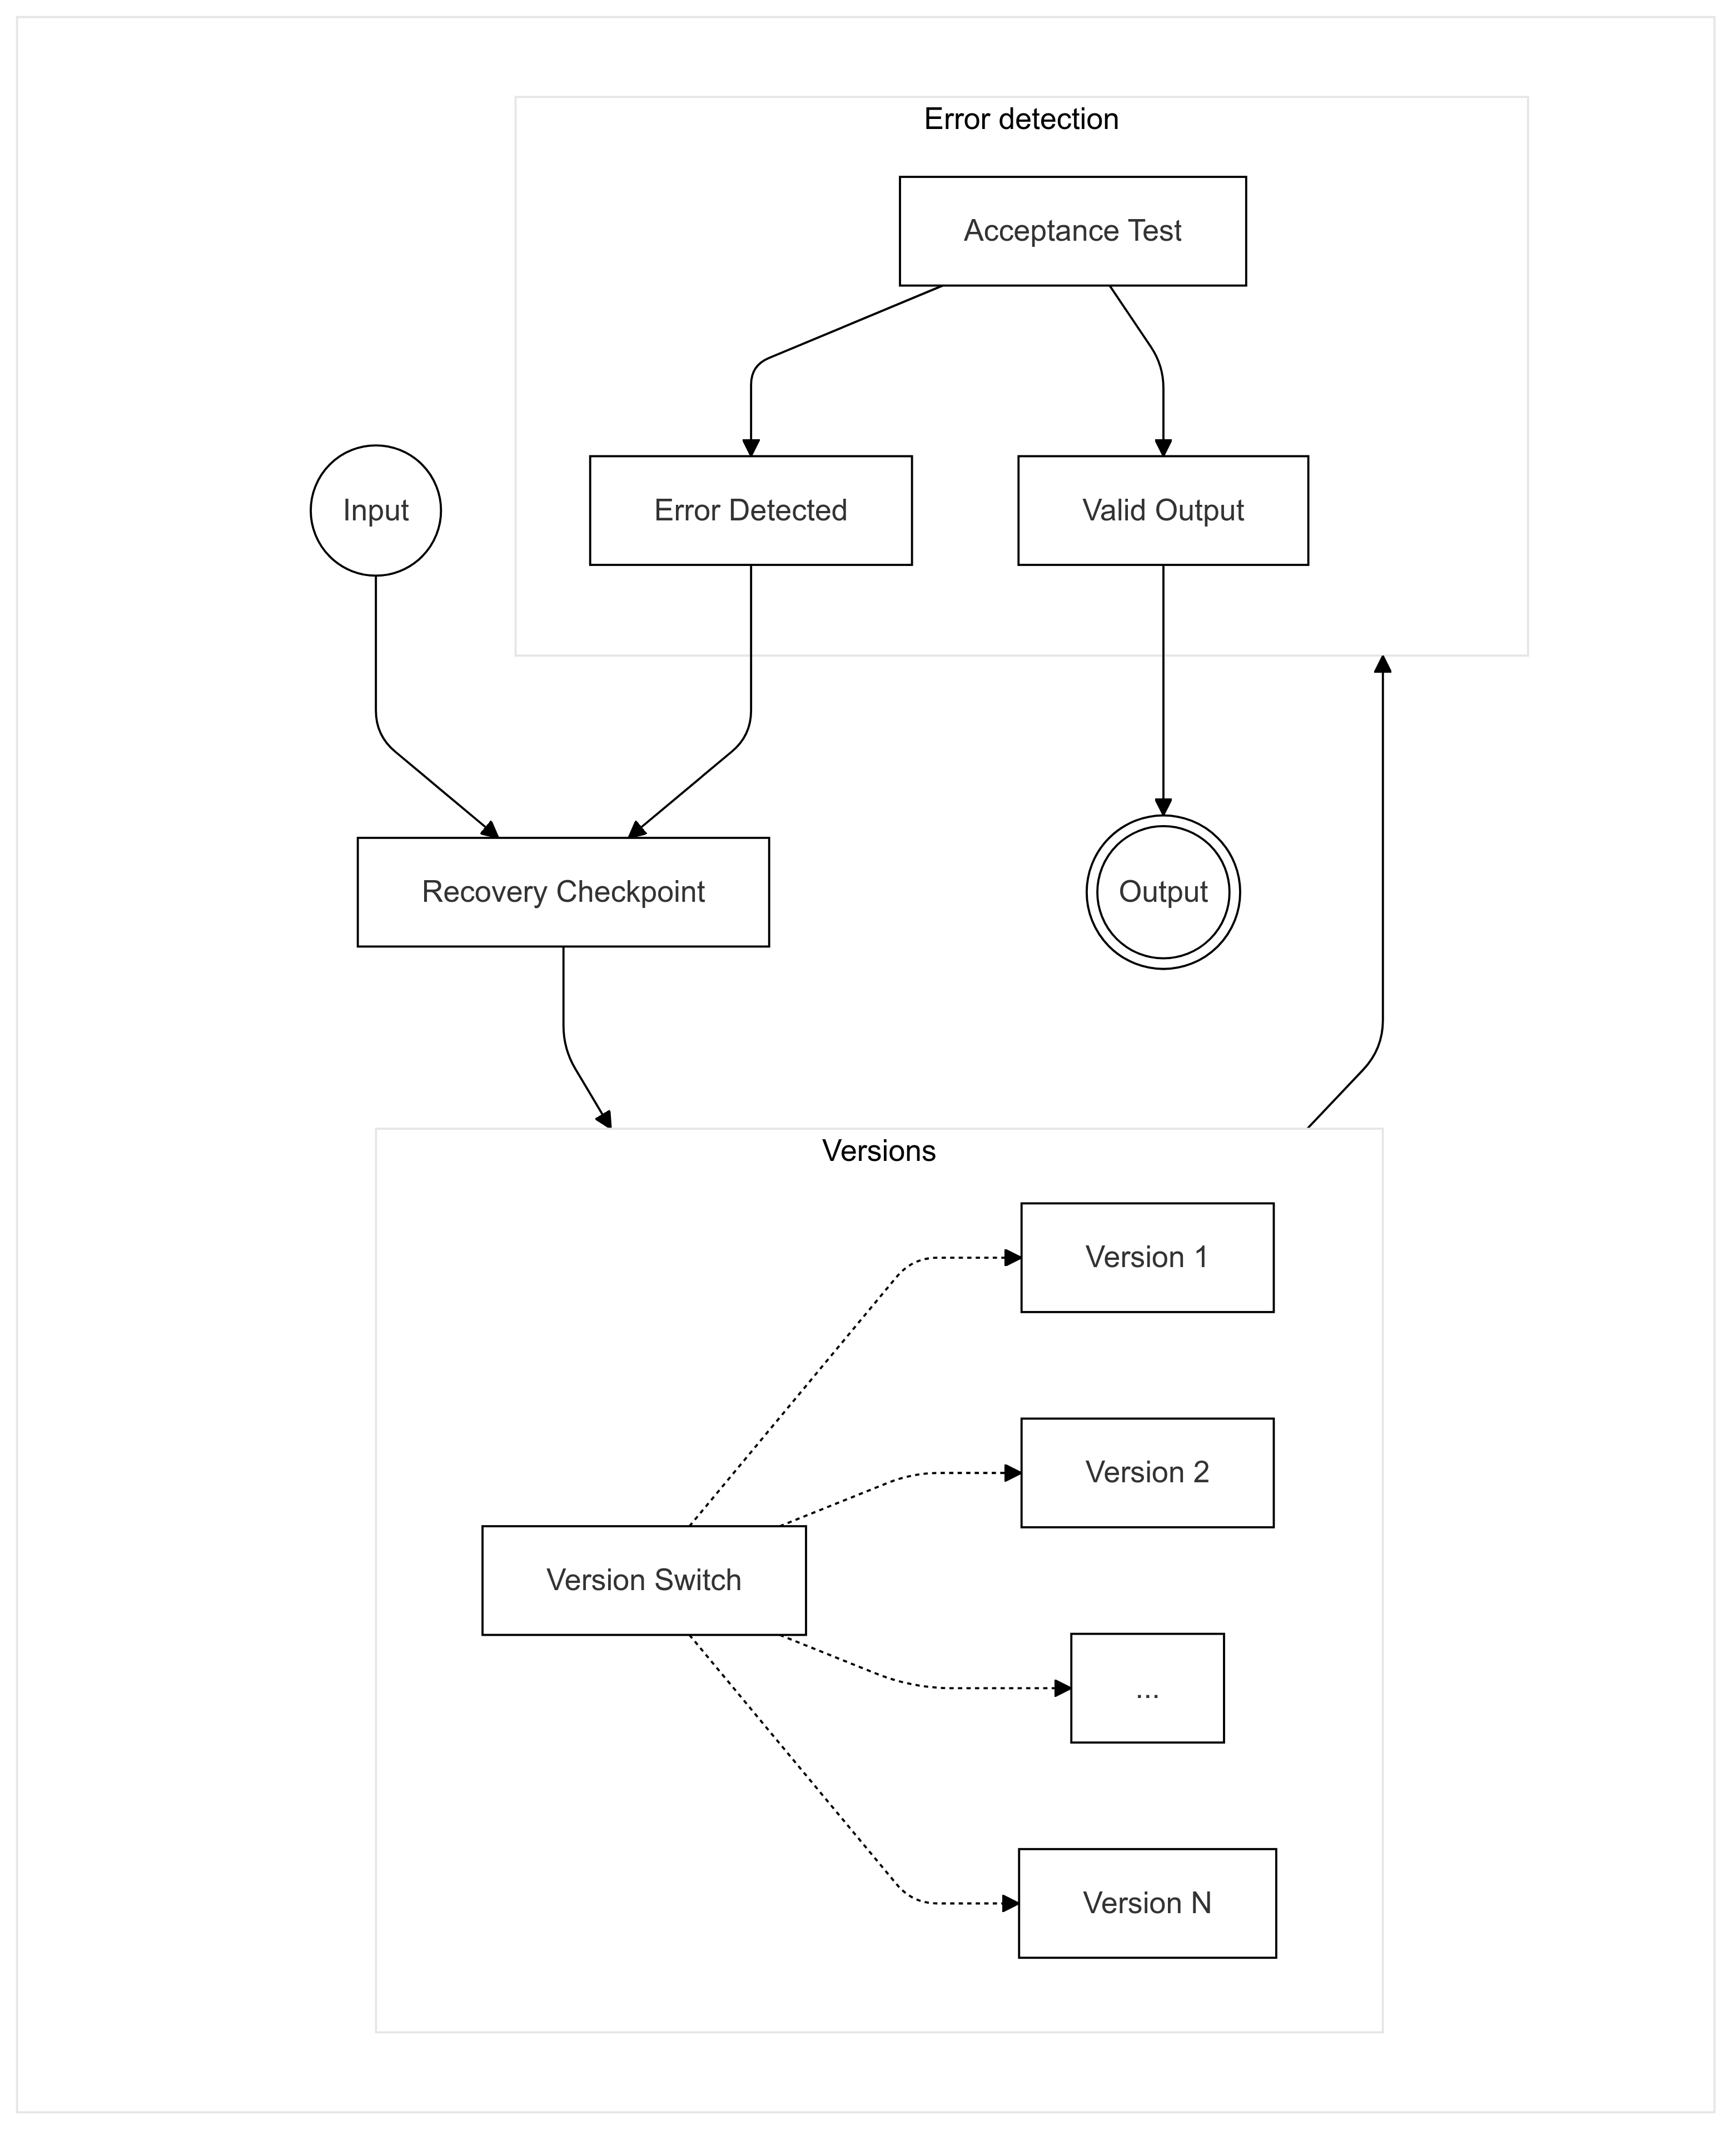
\includegraphics[width=0.9\textwidth]{recovery_blocks/recovery_blocks_01.png}
%     \caption{Recovery Blocks}
%     \label{fig:rec_blo}
% \end{figure}

% \break

Since faults are relatively rare compared to normal execution, this approach often achieves an optimal balance of performance and reliability. By prioritizing efficiency in the primary execution path while incorporating progressively resilient alternatives, recovery blocks can provide dependable fault tolerance without compromising system performance in typical operating conditions. This balance makes recovery blocks a practical solution for systems requiring high availability and reliability.

A consideration for recovery blocks is the utilization of a single shared acceptance check for all the versions. This means that the acceptance check must be implementation agnostic and only consider the inputs and outputs of the version. Although this means easier development and potentially less opportunities for faults given less software design, it also fails to take advantage of version-specialized ways errors could be detected in theory.

A considerable drawback of recovery blocks is its inability to detect faults which might appear as normal execution of the program. As an example, if a bit-flip in the output register of a function results in a value that the acceptance check does not consider invalid an incorrect result will be returned. This error would go undetected without additional checks on top of recovery blocks.

\subsubsection{N-version programming}

N-version programming extends the multi-version technique by running "N" independent versions in parallel or in sequence, hence “N-version” programming. In this approach, each version meeting the same specifications independently performs the task, and the final outcome is determined through a consensus mechanism that evaluates the results from all N executions.

This consensus is usually achieved through a voting algorithm, which aggregates the outputs from each version and selects the result agreed upon by the majority. Selection algorithms are an entire topic of its own covered well by \cite{Aljarbouh_2021}.

This voting approach to handling errors is sometimes referred to as \textbf{fault masking}, since we are not necessarily concerned with detecting an error, but rather getting an acceptable output even in the presence of a fault.

\begin{figure}[hbt!]
    \centering
    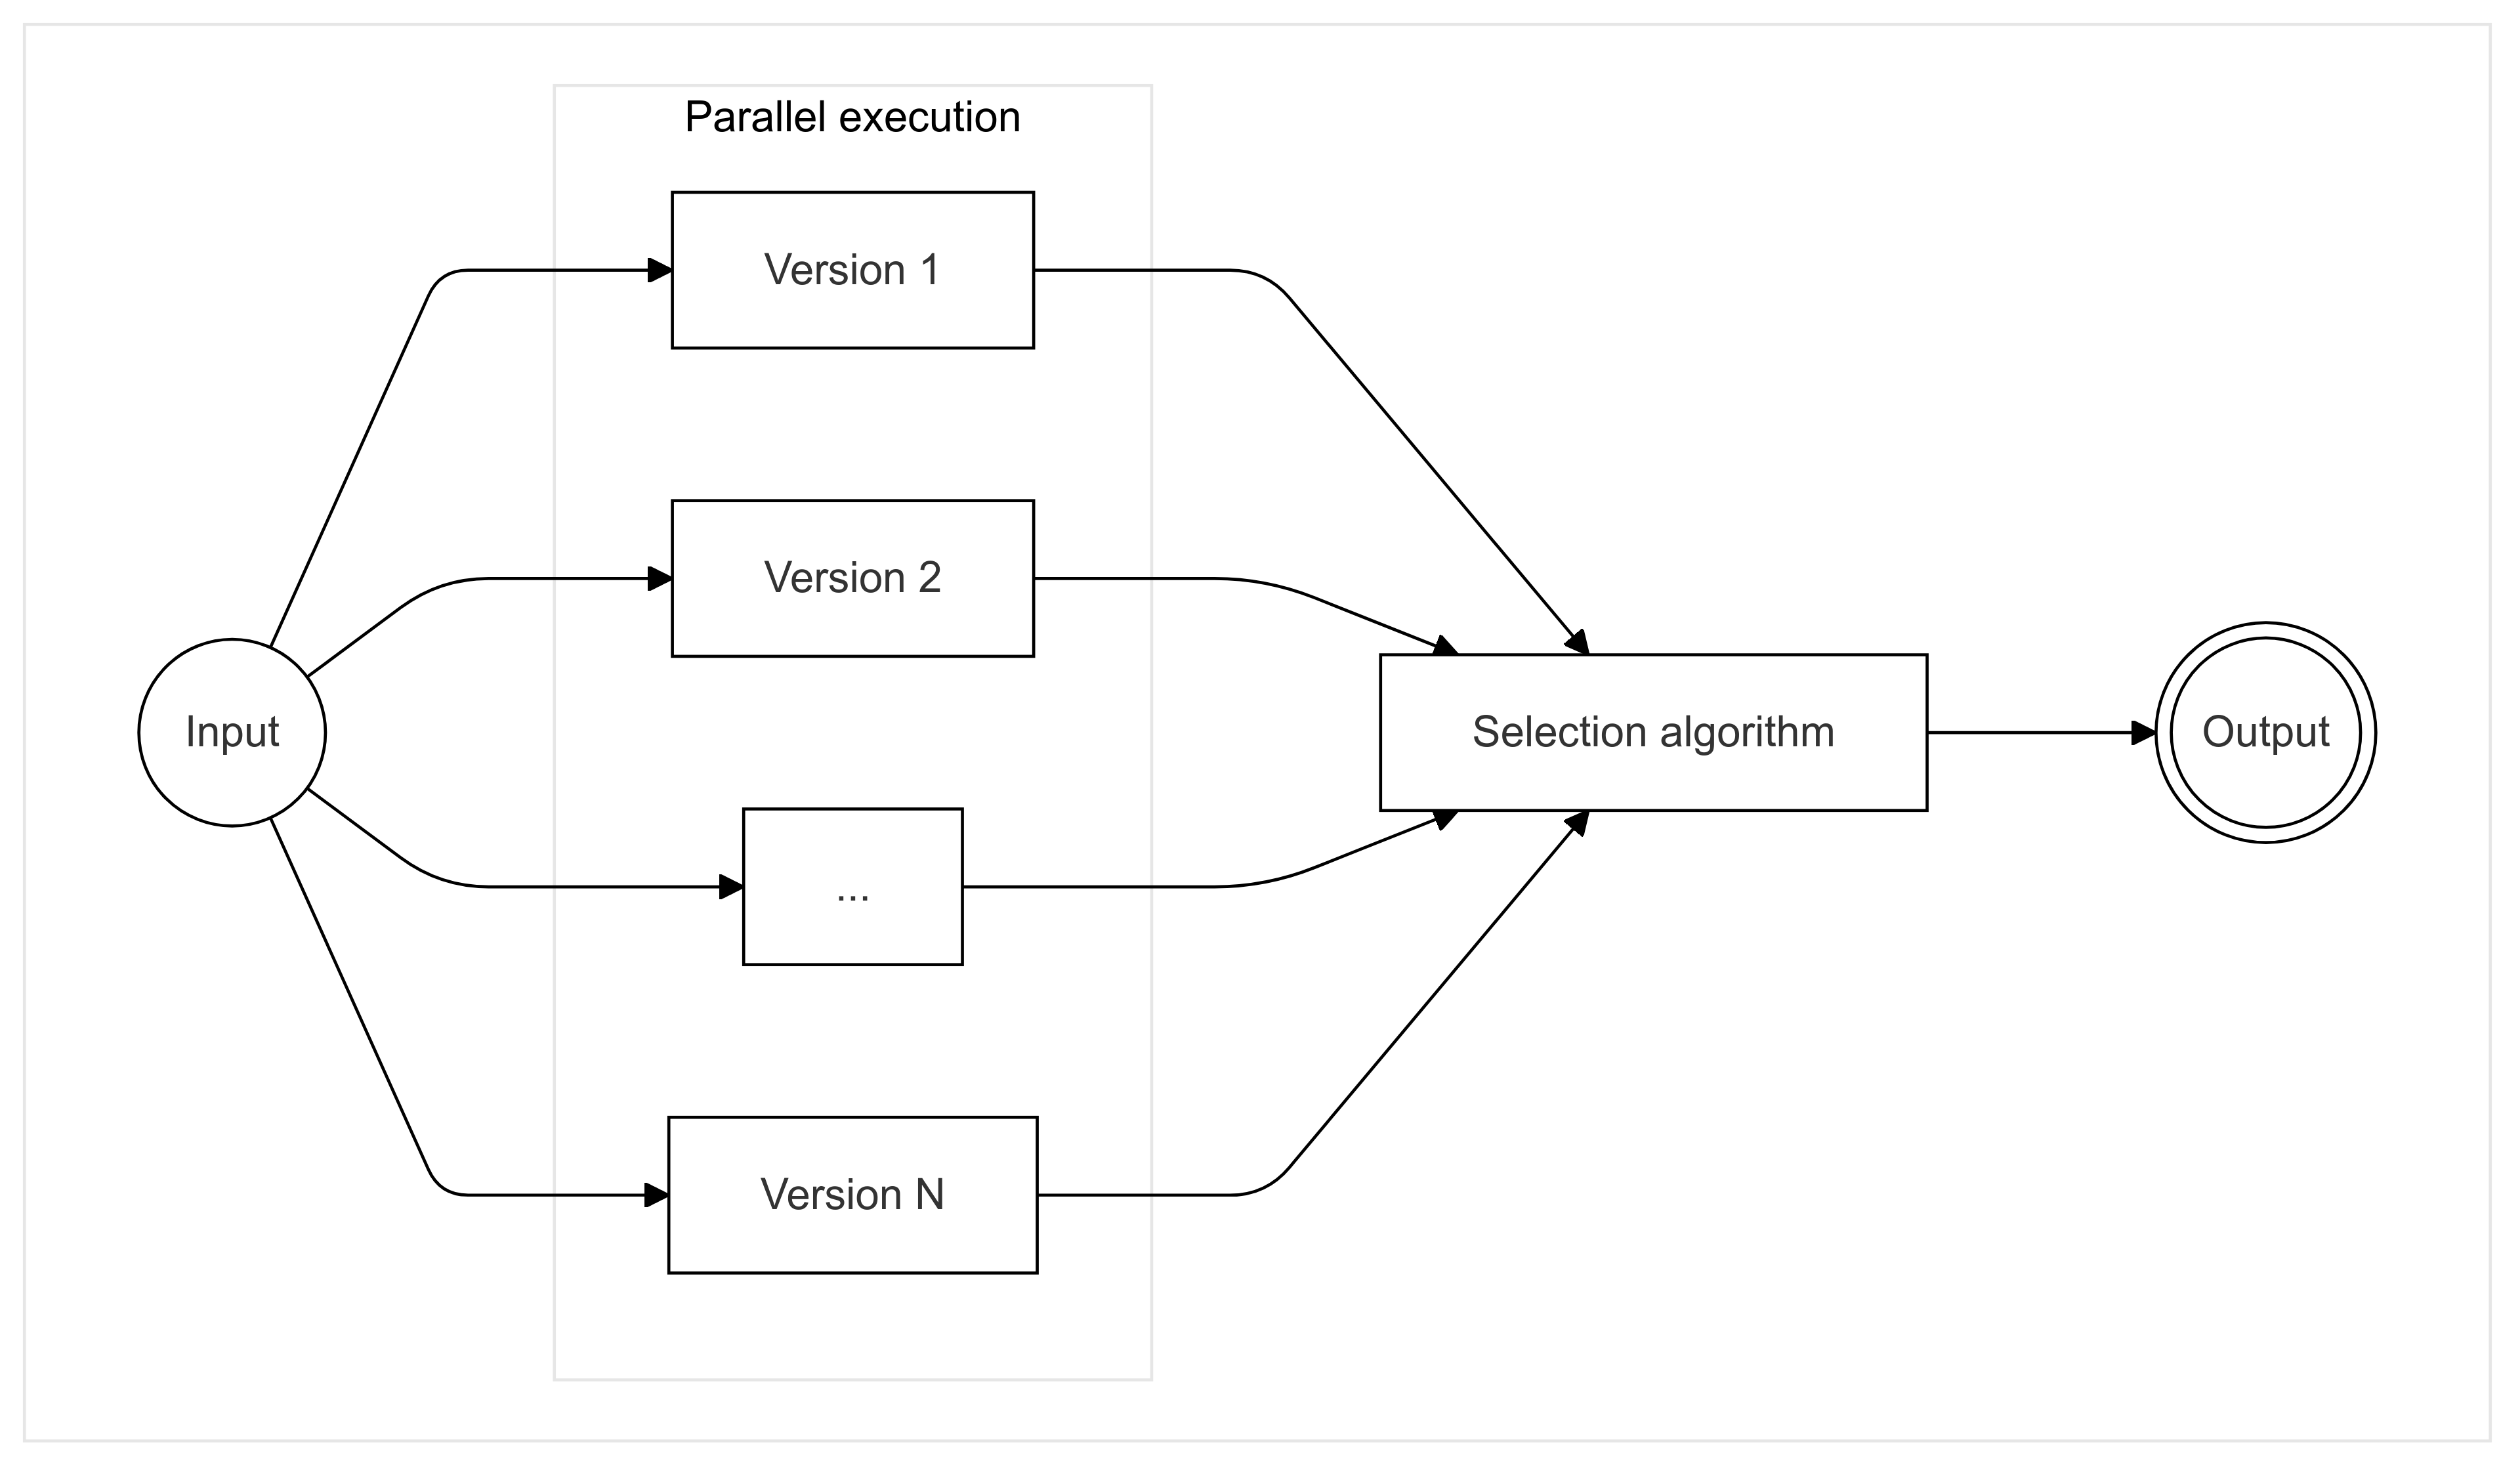
\includegraphics[width=0.9\textwidth]{n_version_prog/n_version_prog.png}
    \caption{N-Version Programming}
\end{figure}

The primary drawback of N-version programming is its requirement to execute all of the versions before determining the final output. This can be highly resource-intensive, especially for large or complex tasks, as it requires significant computational power and memory to run multiple versions simultaneously.

For systems with limited resources, such as embedded systems, this approach can be particularly inefficient. The need to allocate resources for each version can strain the system's capabilities, potentially reducing its overall performance and responsiveness. As a result, while N-version programming enhances fault tolerance and reliability, it may not be suitable for applications where resource constraints are a priority or where processing efficiency is critical.

A consideration for N-version programming is the possibility of an error not being a random event, but rather a function of the input variables \cite{5326}. Therefore, even multiple versions running in parallel could all fail and give erroneous results. This makes the selection algorithm a critical failure point which N-version programming on its own does not address.

\subsubsection{N Self-checking programming}

N Self-checking programming is an extension of the classic N-version programming, where on top of executing multiple versions, each version also contains its own independent acceptance test or recovery block, before the results are passed to the selection logic. The selection logic then selects the "topmost" possible version that reports a correct output.

A version-specialized acceptance check is an interesting addition, as it provides the opportunity to take advantage of the version implementation details. We can specifically tailor the check to consider the inner workings of the version to detect errors and possibly even correct them before proceeding to the selection stage.

The drawback here is the increase in complexity over the more simple recovery blocks which uses a shared acceptance check, or the simple N-version approach which opts for masking instead. By creating more acceptance checks we are introducing more opportunities for errors to manifest, while also spend more resource on development.


\subsubsection{Considerations for multi-version programming}

The primary challenge associated with multi-version programming is the significant effort required to develop, test, and maintain several versions of software that perform the same function. This process can be resource-intensive, leading to increased costs, making it unfeasible for smaller projects or for teams with a limited budget.

To achieve effective multi-version programming, each version must be carefully designed to execute the same task while incorporating distinct failure mechanisms. Ensuring that no two versions fail in the exact same way is very difficult and in practice not always possible.

Research has been conducted into other methods that improve upon the aforementioned multi-version techniques, such as the "t/(n-1)-Variant programming" \cite{589928}. However, the findings do not conclusively prove that the sharp increase in complexity justifies the marginal benefits this or other improved techniques provide.